%****************************************************
%	CHAPTER 6 - System Evaluation
%****************************************************

\chapter{Testing}
\label{ch:ch6}

From Chapter \ref{ch:ch5}, A final set of firmware was developed for two versions of SHARC buoy. The firmware was written for the hardware platforms described in Chapter \ref{ch:ch4} to meet the user requirements (see Chapter \ref{ch:ch3}). This chapter outlines the testing procedure undertaken to validated the device on the following levels.

\begin{enumerate}
	\item low level
	\item Subsystem level
	\item Full system level
	\item Remote test
\end{enumerate}

The testing procedure initiated with low level testing. This was conducted on the firmware with unit tests at each layer (see Figure \ref{fig:soft_arch}) to ensure that the functions written for each subsystem behaved as described in Chapter \ref{ch:ch4}. Then, testing was conducted on a subsystem level to test the base functionality of the module againts the system requirements. Then the system level tests were conducted to test the buoy's response in a controlled environment followed by a Remote level test where the buoy was deployed in an unknown environment to validate the overall performance against the user requirements. Due to time constraints, rigorous data validation tests were not performed. In addition, IMU data and wave simulation testing falls outside the scope of the project.All subsystems are tested as a proof of concept using the unit tests outlined in the design methodology and the subsytem tests outlined in Appendix \ref{tab:UT001} to \ref{tab:UT008}. Finally, due to the 2020 COVID pandemic, final system evaluation of SHARC buoy version 2 could not be conducted during a final research expedition to the Southern Ocean Marginal Ice Zone.  \par 



\section{Subsystem tests}

%Unit test:
%describe and test the base functionality of different firmware modules


In this section, the low level testing is described. As discussed in Sub section \ref{subsec:ch5_timing} Each subsystem has a different data requirement and data rate. The firmware was designed to cater to these requirements ensuring that the correct communication ports were initailised, the correct protocol was used and that an uninterrupted stream of data was created to prevent blocking and timing issues. \par 
 
 \subsection{Unit Tests}
The testing procedure for each subsystem is outlined below. The base functionality of each device is given with the unit test used to verify the functionality. The unit tests were designed IEEE1012\footcite{IEEE_STDVV} as a structural reference to ensure that the outcome of each tests was The unit used  were written to validate the low level functionality of the subsystems and ensure that each module conforms to the outlined specification. Included in each function is a numeric return status describing how the function exited. Table \ref{tab:utsumm} gives an overview of the unit tests shown in Appendix \ref{tab:UT001} to \ref{tab:UT008}.

\begin{table}[H]
	\caption{Objectives of the unit tests defined in Appendix \ref{app:Unittests} showing how the test protocols help validate the firmware in the device peripheral layer.}
	\label{tab:utsumm}
	\setlength{\extrarowheight}{5pt}
	\resizebox{\textwidth}{!}{%
		\begin{tabular}{l >{\raggedright\arraybackslash}m{\textwidth}}
			\hline
			\textbf{Unit test} &\textbf{purpose}\\
			\hline
			\hline
			%initialisation and de initialisation  tests - function routine
			UT001 & Test the initialization and deinitialisation routine for each hardware sub module using the following acceptance criteria The test ensures the firmware can run a successful initialisation routine,the function can recognise when errors occur and the function can detect when the device is offline.\\
			\hline
			%Wireless module data acquisition - modules connecting to satelites
			UT002 & Test the wireless modules line of sight by polling for signal strength or polling the device until it acquires data from a wireless source. \\
			\hline
			%General communication tests
			UT003 & tests the data flow from the microcontroller through to the submodule by polling to transmit or receive data. Test returns an error code based on how the test exited.\\
			\hline
			%Data validation test - functions that validate data
			UT004 & This test is used to verify functions used to safeguard against data corruption by checking that the function can recognise a valid and invalid data based on the implementation of the function.\\
			\hline
			%DMA circular buffer routines
			UT005 &  Tests the UART DMA circular buffer implementation to ensure the stream does not corrupt data and can handle errors.\\
			\hline
			%General functions that interface with the sensor through communication functions
			UT006 & Tests the functions that interface with the sensors to ensure that the data recieved is valid and no errors occur\\
			\hline
			%Error handling
			UT007 & Tests a firmware function under fail conditions to ensure that the function responds by exiting with the appropriate status code without freezing or generating a hard fault.\\
			\hline 
			\hline
		\end{tabular}
	}

\end{table}

%TODO fix the unit tests in the appendix



\subsection{GPS}

\subsubsection{Communication peripheral functionality}

The GPS module communicates through a Universal Asynchronous Receive/Transmission UART port with communication parameters shown in Table \ref{tab:gps_mod}. As discussed in Section \ref{subsec:CH5_gpsss}, a DMA circular buffer was implemented to provide a seamless stream of data directly to non-volatile memory. An input capture channel in slave reset mode was added to the receiver pin to turn the DMA stream off after the line was idle for a defined period. This allowed for a full message of unknown size to be transmitted without polling or generating an interrupt on a byte by byte basis. Table \ref{tab:gps_base} shows the baseline functionality required to achieve this and the methods used to verify this functionality

	\begin{table}[H]
		\centering
		\caption{Baseline functionality of the GPS UART communication module of the firmware and the unit test used to verify this functionality}
		\label{tab:gps_base}
		\setlength{\extrarowheight}{5pt}
		\resizebox{\textwidth}{!}{%
			\begin{tabular}{c >{\raggedright\arraybackslash}m{\linewidth} l}
				\hline
				& \textbf{Base function} & \textbf{Validation} \\
				\hline 
				\hline
				1 &  Initialise UART communication, TIM input capture slave reset and output compare, DMA peripheral to memory stream. & UT001\\
				\hline
				\multirow{2}{*}{2} & \multirow{2}{\linewidth}{Transmit a message through UART DMA stream.} & UT003 \\ && UT006\\
				\hline
					\multirow{3}{*}{3}  &  \multirow{3}{\linewidth}{Receive a message through UART DMA circular buffer.} & UT003\\ && UT005 \\ && UT006\\ 
				\hline
				4 & Handle interrupts generated from UART communication stream. & UT005\\
				\hline
				5 & Handle errors from the data stream. & UT007\\
				\hline
				\hline
			\end{tabular}}
	\end{table}

To ensure the base level functional requirements were met, the device was tested under the conditions outlined in acceptance test AT001 (Table \ref{tab:AT001}). Then, robustness testing was performed using the conditions outlined in acceptance test AT002 Table \ref{tab:AT002} for fail conditions and AT004 for robustness testing Table \ref{tab:AT004}.
\subsubsection{Subsystem functionality}

On a subsystem level, the system needs to know the device is online and working. This can be achieved by requesting an acknowledgement. To do this, the processor transmits an acknowledgement string to the device. If successfilly recieved, the device will either return an ACK-ACK (acknowledge) or ACK-NACK (not acknowledged). No response means the device is offline while a NACK means the device does not recognise the message sent.Then, the device messages and communication parameters need to be configured. The u-blox NEO 7M and NEO M9N come preset with a UART baud rate of 9600 bits/s \cite{UBLOX_M7N_DATA} and 38400 bit/s \cite{UBLOX_M9N_DATA} respectively. The baud rate was increased to 115200 bits/s to allow for faster data reception resulting in a longer idle period between messages allowing for more efficient message detection. Then, the GSA, GLL and ZDA messages must be enabled. Finally, the incoming messages needed to be tested for validity before the data are extracted and placed in an ice drift packet. This results in the following subsystem functionality.

	\begin{table}[H]
	\centering
	\caption{Baseline functionality of the GPS UART communication module of the firmware and the test used to verify subsystem functionality}
	\label{tab:gps_subsys}
	\setlength{\extrarowheight}{5pt}
	\resizebox{\textwidth}{!}{%
		\begin{tabular}{c >{\raggedright\arraybackslash}m{\linewidth} l}
			\hline
			& \textbf{Subsystem function} & \textbf{Validation} \\
			\hline 
			\hline
			1 & Request acknowledgement from the GPS. & UT006\\
			\hline
			2 &  Configure GPS Baudrate to 115200 bit/s & UT006 \\
			\hline
			3 & Configure GPS messages to output ZDA, GLL and GSA messages & UT006\\ 
			\hline
			4 & Determine whether device has acquired satellite signal & UT002\\
			\hline
			5 & Recieve NMEA ZDA, GLL and GSA message strings & UT005\\
			\hline
			6 & Validate and classify message strings & UT004\\
			\hline
			7 & Timeout if no signal acquired & UT007\\
			\hline
			\hline
	\end{tabular}}
\end{table}

Once complete, the full subsystem underwent robustness testing AT004 (Table \ref{tab:AT004}) and low temperature testing AT008 (Table \ref{tab:AT008}). Additionally, a power test  AT007 (Table \ref{tab:AT007}) was performed to ensure the power characteristics matched to those given in the datasheet. Finally the positional data was verified using a reference GPS and accurate epoch time counter.

\subsection{Iridium modem}

\subsubsection{Communication peripheral functionality}

Much like the GPS, the Iridium modem transmits and receives data through a UART port. A circular buffer such as the one for the GPS was implemented for the Iridium modem to allow for efficient data transfer of messages of an unknown length. This would allow for variable-sized messages to be transmitted should any sensors need to be changed or data packets need to be resized. Furthermore, power control was required to keep the modem in a low power state. This was achieved through a digital microcontroller pin connected to the On/Off pin on the modem. The pin needed to stay active low in low power mode to ensure the device was switched off for the full cycle until necessary. This results in the following base functionality:


\begin{table}[H]
	\centering
	\caption{Baseline functionality of the Iridium UART communication peripheral of the firmware and the test used to verify unit functionality.}
	\label{tab:iridium_base}
	\setlength{\extrarowheight}{5pt}
	\resizebox{\textwidth}{!}{%
		\begin{tabular}{c >{\raggedright\arraybackslash}m{\linewidth} l}
			\hline
			& \textbf{Base function} & \textbf{Validation} \\
			\hline 
			\hline
			1 &  Initialise/deinitialise UART communication on the serial port with interrupt generated when the line is idle. & UT001\\
			\hline
			\multirow{2}{*}{2} & \multirow{2}{\linewidth}{Transmit a message through UART DMA stream.} & UT003 \\ && UT006\\
			\hline
			\multirow{3}{*}{3}  &  \multirow{3}{\linewidth}{Receive a message through UART DMA circular buffer.} & UT003\\ && UT005 \\ && UT006\\ 
			\hline
			4 & Handle interrupts from UART commnunication stream & UT005 \\
			\hline
			5 & Handle errors from UART communication stream & UT006 \\
			\hline 
			6 & Control the power mode with a digital output pin & UT008 \\
			\hline
			7 & Receive interrupts from ring alert pin & UT008 \\
			\hline
			\hline
	\end{tabular}}
\end{table}

The base functionality was tested in ideal conditions described in AT001 (Table \ref{tab:AT001}), fault testing in conditions described in AT002 (Table \ref{tab:AT002}) and robustness testing in  AT004 (Table \ref{tab:AT004}).

\subsubsection{Subsystem functionality}

On a subsystem level, the firmware controls the RockBLOCK 9603 modem using AT commands. These are command strings that begin with "AT" and finish with a "$\backslash$r" character. The device comes preconfigured to communicate at 19200 bits/s with no flow control. To ensure the device is working, the microcontroller can request acknowledgement with the command "AT$\backslash$r" which shold return "OK" if successful. The subsystem should therefore be able to interpret the success of a command based on the return function. The modem accepts data in the form of binary or ASCII messages thereby requiring routines to upload data in either ASCII or binary format. Finally, the microcontroller initiates a transmission by sending the command "AT+SBDIX$\backslash$r". The transmission takes 10 seconds to complete before a return status is returned. Finally the device needs to be put to sleep mode to reduce current when inactive and turned on when required. This was done by interfacing with the modem through the digital on-off control pin. This results in the following subsystem functionality:

\begin{table}[H]
	\centering
	\caption{Baseline functionality of the Iridium UART communication peripheral of the firmware and the test used to verify unit functionality.}
	\label{tab:iridium_subsys}
	\setlength{\extrarowheight}{5pt}
	\resizebox{\textwidth}{!}{%
		\begin{tabular}{c >{\raggedright\arraybackslash}m{\linewidth} l}
			\hline
			& \textbf{Subsystem function} & \textbf{Validation} \\
			\hline 
			\hline
			1 &  Request acknowledgement & UT006\\
			\hline
			\multirow{2}{*}{2} & \multirow{2}{*}{Interpret return status*} & UT004\\&& UT005\\
			\hline
			3 &  Upload AT command &  UT006\\
			
			4 & Upload ASCII message & UT006 \\
			\hline
			5 & Upload Binary message & UT006 \\
			\hline 
			6 & Aqcuire network signal & UT002 \\
			\hline
			7 & Initiate satellite transmission & UT006 \\
			\hline
			8 & Handle transmission errors &  UT007\\
			\hline
			\hline
	\end{tabular}}
\end{table}

Once complete, the full subsystem underwent robustness testing AT004 (Table \ref{tab:AT004}) and low temperature testing AT008 (Table \ref{tab:AT008}), a transmission test and a power test  AT007 (Table \ref{tab:AT007}) to confirm the power characteristics and to ensure that the device was turned off during all periods of inactivity.

\subsection{Environmental sensor}
\subsubsection{Communication peripheral functionality}

The microcontroller interfaces with the BMP280 sensor through SPI. As shown in the data requirements, the device will be sampling data from the sensor in short burst reads. A maximum of 24 bytes is transferred at a given time and this occurs when reading the compensation registers \cite{BMP280_Datasheet}. Therefore, the sensor would be operated in a simple polling mode with data read in bursts per the recommendations of \textcite{BMP280_Datasheet} to ensure that data do not arrive fragmented. This would also greatly simplify the communication peripheral functionality which is shown in Table \ref{tab:env_base}. Finally, the software needs to be able to write to transmit data to specific registers on the sensors to control the configuration, output type and power mode

\begin{table}[H]
	\centering
	\caption{Baseline functionality of the BMP280 SPI communication peripheral of the firmware and the tests used to verify unit functionality.}
	\label{tab:env_base}
	\setlength{\extrarowheight}{5pt}
	\resizebox{\textwidth}{!}{%
		\begin{tabular}{c >{\raggedright\arraybackslash}m{\linewidth} l}
			\hline
			& \textbf{Base function} & \textbf{Validation} \\
			\hline 
			\hline
			1 &  Initialise/deinitialise SPI communication & UT001\\
			\hline
			2 & Read from an 8-bit register & UT003 \\
			\hline
			3 & write to an 8-bit register & UT003\\
			\hline
			4 & Validate incoming data & UT004\\
			\hline
			5 & Handle errors. & UT007\\
			\hline
			\hline
	\end{tabular}}
\end{table}

The functional requirements were further validated using test protocols AT001 (Table \ref{tab:AT001}) for connectivity testing , AT002 (Table \ref{tab:AT002})  for fault testing and AT004 (Table \ref{tab:AT004}) for robustness testing. This ensured that the baseline functional requirements were met.

\subsubsection{Subsystem functionality}  

On a subsystem level, interactions with the BMP280 occur by reading and writing to the onboard registers. The device can be tested for functionality by reading the value from the \textit{whoami} register. This chec ensures the device is online and functional. Furthermore, the BMP280 is fully programmable and can be configured by writing to the \textit{ctrl\_meas} and \textit{config} registers at memory addresses 0xF4 and 0xF5 respectively. When a conversion takes place, the status register bits are set to 1 to signify that a conversion is taking place. Being able to read this register will allow for hte microcontroller to synchronize with the BMP280 measurement cycle. Finally the factory calibration values need to be read and calculated to calculate the temperature and pressure values from their raw ADC values. This results in the following Subsystem functionality shown in Table \ref{tab:env_subsys}.

\begin{table}[H]
	\centering
	\caption{Baseline functionality of the BMP280 SPI communication peripheral of the firmware and the tests used to verify unit functionality.}
	\label{tab:env_subsys}
	\setlength{\extrarowheight}{5pt}
	\resizebox{\textwidth}{!}{%
		\begin{tabular}{c >{\raggedright\arraybackslash}m{\linewidth} l}
			\hline
			& \textbf{Subsystem function} & \textbf{Validation} \\
			\hline 
			\hline
			1 & Read device ID. & UT004\\	\hline
			2 & Configure device.& UT006 \\ \hline
			3 & Set Power mode. & UT006\\ \hline
			4 & Trigger conversions.& UT006\\ \hline
			5 & Read measurement status. & UT006\\ \hline
			6 & Read raw ADC values. & UT006\\ \hline
			7 & Read factory calibration parameters.& UT006\\ \hline
			8 & Calculate Pressure and temperature from ADC values. &UT004 \\ \hline
			9 & Handle errors.& UT007 \\
			\hline
			\hline
	\end{tabular}}
\end{table}

During testing, the sensor was configured in weather station mode which was recommended for environmental monitoring with sample rates greater than once per second \cite{BMP280_Datasheet}. These configuration parameters are shown in Table \ref{tab:bmp_param}

\begin{table}[H]
	\centering
	\caption{Table showing the configuration parameters for the BMP280 environmental sensor for the final version of the buoy firmware.}
	\label{tab:bmp_param}
	\begin{tabular}{l c}
		\hline
		\hline
		Temperature oversample & 1\\
		\hline
		Pressure oversample & 1\\
		\hline
		Infinite impulse response (IIR) coefficients & off\\
		\hline
		Measurement mode & Forced \\
		\hline
		Standby time [s] & off\\
		\hline
		\hline
	\end{tabular}
\end{table}

 Placing the device in forced conversion mode required the microcontroller to manually trigger a conversion. The standby time measures the time between each measurement completed by the sensor. Since the device is in forced mode, this parameter is not used. When the device was not performing a measurement, it was in sleep mode which conserved power. The subsystem was fully tested using AT004 (Table \ref{tab:AT004}) and AT008 (Table \ref{tab:AT008}) to ensure the device performed under stress and in low temperature. Measurements were validated by placing the buoy in a controlled environment and comparing the measured temperature and pressure to an accurate reference.
\subsection{Power monitor}


\subsubsection{Communication peripheral functionality}

The INA219 communicates with the microcontroller over I$^2$C. Unlike the BMP280 or the MPU6050, this device has a 16-bit architecture requiring a two-byte read of data. Data are sampled in 30 minute intervals with a single data point read from this device for shunt voltage, bus voltage, current and power. Therefore, in line with the approach taken with the BMP280, the micro controller will read and write from the sensor in polling mode. The device begins communication upon reception of an address b Any errors that occur during communication result in error codes returned that give more information about the type of issue encountered. The baseline functionality for the INA219 power monitor is shown in Table \ref{tab:pwr_base}.

\begin{table}[H]
	\centering
	\caption{Baseline functionality of the INA219 I$^2$C communication peripheral of the firmware and the tests used to verify unit functionality.}
	\label{tab:pwr_base}
	\setlength{\extrarowheight}{5pt}
	\resizebox{\textwidth}{!}{%
		\begin{tabular}{c >{\raggedright\arraybackslash}m{\linewidth} l}
			\hline
			& \textbf{Subsystem function} & \textbf{Validation} \\
			\hline 
			\hline
			1 & Initialise/deinitialise I$^2$C peripheral. & UT001\\	\hline
			2 & Transmit data to a 16-bit register on the sensor.& UT003 \\ \hline
			3 & Read data from a 16-bit register on the sensor. & UT003\\ \hline
			4 & Validate incoming data& UT004\\ \hline
			5 & Handle errors & UT007\\ \hline
			\hline
			\hline
	\end{tabular}}
\end{table}

The functional requirements were further validated using test protocols AT001 (Table \ref{tab:AT001}) for connectivity testing , AT002 (Table \ref{tab:AT002})  for fault testing and AT004 (Table \ref{tab:AT004}) for robustness testing. This ensured that the baseline functional requirements were met.
\subsubsection{Subsystem functionality}

The microcontroller initiates communication with The INA219 by transmitting an address byte to the sensor. This address byte is set by the pins A1 and A0 \cite{INA219} and can take on 16 values. For this version, both pins were set to ground generating an address byte of 0b1000 0000 (0x80).  Transmitting this address byte allows the microcontroller to additionally check if the device is online. The device also comes preloaded with a configuration value in the register which resets during a power cycle \cite{INA219}. This value can also be used to chec for previous configurations or corrupted chips. The INA219 is also the only sensor in the SHARC buoy system to require a manual calibration before use. The process for calibrating this sensor is given in \cite{INA219} and was implemented in the firmware to calibrate the sensor for 16V bus range and a maximum 1.2 A. The function outputs an LSB value that scales the ADC readings from the sensor to match the actual power information being sampled. The device is fully programmable. Therefore, sensor configuration functions were written to easily configure the sensor through a parametric function. These functions were validated by reading the registers after a value was written to it to see if it had accepted the new configurations. Finally, the device was configured for a maximum bus range voltage of 16V with an ADC resolution of 12 bits for both shunt and bus voltages. The device was also configured to opperate in triggered mode where the microcontroller manually triggers a single measurement in the device. Once complete, the device is placed into sleep mode. This functionality is shown in Table \ref{tab:pwr_subsys}.

\begin{table}[H]
	\centering
	\caption{Subsystem functionality of the INA219 I$^2$C communication peripheral of the firmware and the tests used to verify unit functionality.}
	\label{tab:pwr_subsys}
	\setlength{\extrarowheight}{5pt}
	\resizebox{\textwidth}{!}{%
		\begin{tabular}{c >{\raggedright\arraybackslash}m{\linewidth} l}
			\hline
			& \textbf{Subsystem function} & \textbf{Validation} \\
			\hline 
			\hline
			1 & Request acknowledgment from the sensor. & UT004\\	\hline
			2 & Configure device.& UT006 \\ \hline
			3 & Calibrate device& UT006\\ \hline
			4 & Trigger conversion & UT006\\ \hline
			5 & Read data and convert from ADC value & UT006\\
			\hline
			\hline
	\end{tabular}}
\end{table}

The subsystem was fully tested using AT004 (Table \ref{tab:AT004}) and AT008 (Table \ref{tab:AT008}) to ensure the device performed under stress and in low temperature. Power,  current and voltage values were verified by connecting the sensor across a load of known resistance and voltage and measuring the values.
\subsection{Flash chips}

\subsubsection{Communication peripheral functionality}
The library for the AT45DB641E flash chips was written by N. Bowden and was designed to allow the microcontroller to interface with multiple flash chips on the same SPI port. each chip had a chip select pin connected to a unique GPIO pin on the microcontroller. This allowed for individual chips to be selected. This requires the microcontroller to keep track of which chips are connected to the lines in order to keep careful control over the flow of data between the chips. As a safeguard, the write protect pins of each chip were connected to a single control pin. This would prevent data from being corupted or unexpectedly overwritten. The flash chips communicate via SPI requiring the library to have the baseline functionality shown in Table \ref{tab:flash_comm}.

\begin{table}[H]
	\centering
	\caption{Baseline functionality of the AT45DB641E flash chips SPI  communication peripheral of the firmware and the tests used to verify unit functionality.}
	\label{tab:flash_comm}
	\setlength{\extrarowheight}{5pt}
	\resizebox{\textwidth}{!}{%
		\begin{tabular}{c >{\raggedright\arraybackslash}m{\linewidth} l}
			\hline
			& \textbf{Subsystem function} & \textbf{Validation} \\
			\hline 
			\hline
			1 & Initialise/Deinitialise SPI peripheral & UT001\\	\hline
			2 & Initialise chip select and write protect pins.& UT001 \\ \hline
			3 & SPI  write to a memory location. & UT003\\ \hline
			4 & SPI read from a memory location.& UT003\\ \hline
			5 & Enable/disable chips & UT008\\ \hline
			6 & Enable/disable write protect & UT008 \\ \hline
			7 & Handle errors & UT007\\ \hline
			\hline
			\hline
	\end{tabular}}


\end{table}
The functional requirements were further validated using test protocols AT001 (Table \ref{tab:AT001}) for connectivity testing , AT002 (Table \ref{tab:AT002})  for fault testing and AT004 (Table \ref{tab:AT004}) for robustness testing. This ensured that the baseline functional requirements were met.

\subsubsection{Subsystem functionality}

Each chip is monitored by the firmware to ensure that there is sufficient memory and the devices are online. The chips are given a number and a status written to the very first byte of memory on each chip When one chip reaches full capacity,the status is set to full and the next chip is formatted and set to to active. When the last chip is full, the first chip is selected again and the memory cycle restarts If a memory chip suddenly stops working, the software will find the next working chip in order and set that to active. This method was tested by taking chips offline one at a time and writting to the last page of memory in the chip. This method forms a circular data buffer The number of the active chip is stored in the first byte of the 32 bit Back up registers in the RTC.The primary role of the flash chips is to provide a permanent, ordered storage solution to large data sets. The firmware was designed to manage the data by constantly tracking the amount of data saved to memory and the latest occupied memory address. Memory addresses are three bytes long and the memory address with the corresponding chip number These values are stored in the RTC Back up register. Packets of data are written to memory at the end of every sample routine in sequential order increment the memory address by the set number of bytes. The firmware reads the chip data by calculating the difference in the starting memory address and the last known memory address to determine th number of bytes to read and performing a burst read starting at the start address. This subsystem functionality is shown in Table \ref{tab:subsys_flash}

\begin{table}[H]
	\centering
	\caption{Subsystem functionality of the AT45DB641E flash chips SPI communication peripheral of the firmware and the tests used to verify unit functionality.}
	\label{tab:subsys_flash}
	\setlength{\extrarowheight}{5pt}
	\resizebox{\textwidth}{!}{%
		\begin{tabular}{c >{\raggedright\arraybackslash}m{\linewidth} l}
			\hline
			& \textbf{Subsystem function} & \textbf{Validation} \\
			\hline 
			\hline
			1 & Read chip status & UT004\\	\hline
			2 & Set chip status.& UT006 \\ \hline
			3 & Get memory address & UT006\\ \hline
			4 &Set memory address& UT006\\ \hline
			5 & Read Chip Data & UT006\\ \hline
			6 & Write Chip Data & UT006 \\ \hline
			7 & Delete Chip Data& UT006\\ \hline
			8 & Get active chip & UT005\\ \hline
			9 & Set active chip& UT007\\ \hline
			10 & Handle errors & UT007\\ \hline
			\hline
			\hline
	\end{tabular}}
\end{table}

The functional requirements were further validated using test protocols AT001 (Table \ref{tab:AT001}) for connectivity testing , AT002 (Table \ref{tab:AT002})  for fault testing and AT004 (Table \ref{tab:AT004}) for robustness testing.
\subsection{IMU}

\subsubsection{Communication peripheral functionality}
The IMU communicates with the microcontroller via I$^2$C. The firmware transmitted data via polling methods. However, due to the long sample period required by the IMU (see Chapter \ref{ch:ch5}), this method would not be viable as it would block the CPU responding to other critical functions (See Section \ref{subsec:ch5_asynch}). A decision was made to use an interrupt based sampling method by setting an external interrupt line on the microcontroller and connecting it to the interrupt pin on the IMU. Therefore the baseline functionality for this device can be shown in Table \ref{tab:base_imu} 

\begin{table}[H]
	\centering
	\caption{Baseline functionality of the Iridium UART communication peripheral of the firmware and the test used to verify unit functionality.}
	\label{tab:base_imu}
	\setlength{\extrarowheight}{5pt}
	\resizebox{\textwidth}{!}{%
		\begin{tabular}{c >{\raggedright\arraybackslash}m{\linewidth} l}
			\hline
			& \textbf{Base function} & \textbf{Validation} \\
			\hline 
			\hline
			1 &  Initialise/deinitialise I$^2$C & UT001\\
			\hline
			2 & Initalise/deinitialse GPIO pin for digital input and External interrupt line & UT001\\
			\hline
			3 & Write data to 8-bit register on the sensor & UT003\\
			\hline
			4 & Read data from an 8-bit register on the senor & UT003\\
			\hline
			5 & Recieve data in an interrupt-based sample stream& UT005\\
			\hline
			6 & Handle interrupts & UT005 \\
			\hline
			7 & Handle errors & UT007 \\
			\hline
			\hline
	\end{tabular}}
\end{table}

\subsubsection{Subsystem functionality}
The IMU is fully programmable and requires functions to set the Sample rate, power mode, digital filter and the full scale resolution. To verify that the device had been configured, the registers were read to ensure the data in the register matched the byte that had just been written. To verify that the sensor was online, a function was created to read the device id and ensure it matched the value in \textcite{mpu6050}. To verify the sensor was functional, a self test was performed. This is a built in feature that can be activated by writing to the Self Test register. During this process, a value is produced which is measured relative to the factory trim values preloaded in the device. The test is passed if the difference falls within the parameters specified by \textcite{mpu6050}. In Section \ref{sec:dm}, the IMU was configured to output enough data to fit into a single transmission buffer (336 bytes). A single sample of the 6 axes results in a total of 12 bytes per sample. An interrupt would be generated on the interrupt line which triggered the processor to perform a burst read of the acceleramoter and gyroscope data registers on the device. The data was saved to a buffer and the interrupt would be cleared. The device was configured for a 5Hz sample rate and a full scale resolution of $\pm$2 g for the accelerometer and $\pm$ 500$\degree$ s$^{-1}$  for the gyroscope. The digital low pass filter was activated to remove High frequency noise and was set to a bandwidth of 94Hz. Hence, the subsystem functionality is shown in Table \ref{tab:subsys_imu}. 

\begin{table}[H]
	\centering
	\caption{Subsystem functionality of the MPU6050 6 dof IMU and the tests used to verify subsystem functionality.}
	\label{tab:subsys_imu}
	\setlength{\extrarowheight}{5pt}
	\resizebox{\textwidth}{!}{%
		\begin{tabular}{c >{\raggedright\arraybackslash}m{\linewidth} l}
			\hline
			& \textbf{Subsystem function} & \textbf{Validation} \\
			\hline 
			\hline
			1 & Read sensor ID & UT006\\	\hline
			2 & Perform self test& UT009 \\ \hline %add validation function to unit test
			3 & Configure accelerometer & UT003\\ \hline  
			4 & Configure gyroscope & UT003\\ \hline
			5 & Set sample rate & UT003\\ \hline
			6 & Configure interrupt pin & UT008 \\ \hline
			7 & Configure low pass filter bandwidth & \\ \hline
			8 & Read raw gyroscope axis& UT003 \\ \hline
			9 & Read raw accelerometer axis & UT003 \\ \hline
			10 & Calculate acceleration& UT004\\ \hline 
			11 & Calculate angular velocity & UT004\\ \hline
			12 & Handle errors & UT007\\ \hline
			\hline
			\hline
	\end{tabular}}
\end{table}
The subsystem was fully tested using AT004 (Table \ref{tab:AT004}) and AT008 (Table \ref{tab:AT008}) to ensure the device performed under stress and in low temperature. However, IMU data handling falls outside the scope of this thesis and therefore wasnt tested further. 

\section{System Tests}
\label{sec:ch4_systests}

The system tests were conducted using version two of the SHARC buoy system. For these tests the following sensors were enabled for ice drift and diagnostic measurements.

\begin{enumerate}
	\item u-blox NEO M9N
	\item Bosch Sesnortech BMP280
	\item Texas Instruments INA219
\end{enumerate}

These sensors were sampled at an interval of 30 minutes with the device placed into standby mode in between samples. During the test, the LED was configured to flash on when the device successfully activated a sensor. This LED was also configured to turn on when the buoy was in an active state. Finally debugging and diagnostic information was transferred to a computer through a USB cable. This data was timestamped and recorded to a log. Finally, the following sensors were enabled for wave in ice measurements. 
\begin{enumerate}
	\item TDK Invensense MPU6050
\end{enumerate}

the MPU6050 was set to sample every 2 hours by synchronising the sample interval to four ice drift samples. At the end of the 2 hour period, the transmission routine was completed. All sensors were configured as described in the subsystem tests and the following tests were performed.

\subsection{SYS001 accelerated system test}

\subsubsection{Scope}
The accelerated system test aimed to test the systems ability to complete a single cycle described in Chapter \ref{ch:ch5}. This will verify the performance of the system against AT005 (Table \ref{tab:AT005}).
\subsubsection{Protocol}

The ice drift sample interval was set to 10 seconds with transmission occurring after four sample sessions. Batteries are inserted and the device is placed inside the enclosure. The buoy was placed in an area with an unobstructed view of the sky. The system was left to run for a single cycle from initialisation. Data was recorded from the buoy through a serial debug output to USB which connected to a serial monitor running on a computer to record and timestamp the output.\\
\subsubsection{Configurations}
GPS data was sampled at 1 Hz until a full packet of datum, diagnostic and positional information was achieved. The BMP280 and INA219 current sensors were sampled once per sample period and the MPU6050 was sampled at 5 Hz for 67.2 seconds.
\subsubsection{Results}

A sample of the Buoy output from SYS001 system test is shown in Table \ref{tab:SYS001_res1}. Data is timestamped debug outputs from the buoy showing the behavior of the system as well as the subsystems. Environmental data is shown in 16 bit signed integer representation as discussed in Chapter \ref{ch:ch5}.

\begin{table}[H]
	\centering
	\caption{System output during an accelerated test as described in SYS001. data output occurs over the period from initialation to first sample and sleep with a failed GPS signal acquisation.}
	\label{tab:SYS001_res1}
	\setlength{\extrarowheight}{5pt}
	\resizebox{\textwidth}{!}{%
	\begin{tabular}{l}
	\hline
	\hline
	"11/21/2020 7:47:40 PM",Warning! Device encountered a Brown Out. Exiting Program...\\ \hline 
	"11/21/2020 7:47:40 PM",Software Reset Detected. Initializing main program...\\ \hline 
	"11/21/2020 7:47:40 PM",Setting Up Flash Chips...\\ \hline 
	"11/21/2020 7:47:40 PM",Allocating Chip Statuses...\\ \hline 
	"11/21/2020 7:47:40 PM",Chip 1 Status: 1\\ \hline 
	"11/21/2020 7:47:40 PM",Chip 2 Status: 2\\ \hline 
	"11/21/2020 7:47:40 PM",Chip 3 Status: 3\\ \hline 
	"11/21/2020 7:47:40 PM",Chip 4 Status: 3\\ \hline 
	"11/21/2020 7:48:02 PM",Error Connecting To Modem\\ \hline 
	"11/21/2020 7:48:02 PM",Environmental Sensor Online!\\ \hline 
	"11/21/2020 7:48:02 PM",Current Monitor Offline!\\ \hline 
	"11/21/2020 7:48:02 PM",IMU Online\\ \hline 
	"11/21/2020 7:48:02 PM",Device Online!\\ \hline 
	"11/21/2020 7:48:02 PM",Current State: RESET 	 Next State: SAMPLE\\ \hline 
	"11/21/2020 7:48:02 PM",Current State: SAMPLE 	 Next State: SLEEP\\ \hline 
	"11/21/2020 7:48:19 PM",GPS Online! Acquiring Signal...\\ \hline 
	"11/21/2020 7:48:49 PM",Failed to Acquire Signal\\ \hline 
	"11/21/2020 7:48:49 PM",Logging Data...\\ \hline 
	"11/21/2020 7:48:49 PM",local time: 1605988066, position: 0.000000 Lat, 0.000000 long\\ \hline 
	"11/21/2020 7:48:49 PM",HDOP = 99.99, 	 PDOP = 99.99, VDOP = 99.160\\ \hline 
	"11/21/2020 7:48:49 PM",Number of Satellites 0, Fix Type = 1\\ \hline 
	"11/21/2020 7:48:49 PM",Environmental Sensor Online!\\ \hline 
	"11/21/2020 7:48:49 PM",Temp = 2346°C 	 Pressure = 101285 Pa \\ \hline 
	"11/21/2020 7:48:49 PM",Successfully saved drift data to chip 1\\ \hline 
	"11/21/2020 7:48:49 PM",Current State: SLEEP 	 Next State: SAMPLE\\ \hline 
	"11/21/2020 7:48:49 PM",Good Night! \\ 
	\hline 
	\hline
	\end{tabular}
	}	
\end{table}

Figure \ref{tab:SYS001_res1} shows an accelerated test from Initialisation to the end of the first sample cycle and sleep mode. The system was unable to acquire a GPS signal and therefore timed out while resuming normal operations. A successful GPS signal acquisition is shown below during the phases: first wake up to the end of second sample.

\begin{table}[H]
	\centering
	\caption{System output during an accelerated test as described in SYS001. data output occurs over the period from first wake up to the end of second sample with successful GPS signal acquisition.}
	\setlength{\extrarowheight}{5pt}
	\setlength{\textwidth}{5pt}
		\begin{tabular}{l}
			\hline
			\hline
		"11/21/2020 8:18:48 PM",Current State: SAMPLE 	 Next State: SLEEP\\ \hline 
		"11/21/2020 8:18:50 PM",GPS Online! Acquiring Signal...\\ \hline 
		"11/21/2020 8:18:58 PM",Logging Data...\\ \hline 
		"11/21/2020 8:18:58 PM",local time: 1605989870, position: -3357.781250 Lat, 1822.458984 long\\ \hline 
		"11/21/2020 8:18:58 PM",HDOP = 7.50, 	 PDOP = 1.86, VDOP = 7.160\\ \hline 
		"11/21/2020 8:18:58 PM",Number of Satellites 4, Fix Type = 3\\ \hline 
		"11/21/2020 8:18:58 PM",Environmental Sensor Online!\\ \hline 
		"11/21/2020 8:18:58 PM",Temp = 2391°C 	 Pressure = 101215 Pa \\ \hline 
		"11/21/2020 8:18:58 PM",Successfully saved drift data to chip 1\\ \hline 
		"11/21/2020 8:18:58 PM",Current State: SLEEP 	 Next State: SAMPLE\\ \hline 
		"11/21/2020 8:18:58 PM",Good Night! \\ \hline 
		"11/21/2020 8:48:57 PM",Current State: SAMPLE 	 Next State: SLEEP\\ \hline  
		\hline
		\end{tabular}
\end{table}

\subsection{SYS002 power test}
\subsubsection{Scope}
The power test aims to verify to test power consumption characteristics of the buoy to determine the survivability of the device in standard operating conditions to verify the software robustness against AT007 (Table \ref{tab:AT007}).
\subsubsection{Protocol}
 The buoy was connected to a power source with all sensors enabled. The device sampling interval was set to 30 minutes between drift measurements as described above. The device was connect to an Agilent bench top power supply set to output a constant 7.2 V. A data logger was connected to the INA219 sensor and configured to sample current, supply voltage and power consumption. The test ran for a single cycle sampling data at a constant 1 Hz. The logger outputted data to a serial through USB to a computer which recorded the data. The test was completed after a single uninterrupted firmware cycle. This configuration is shown in Figure \ref{fig:pwrtest}.
 \begin{figure}[H]
 	\centering
 	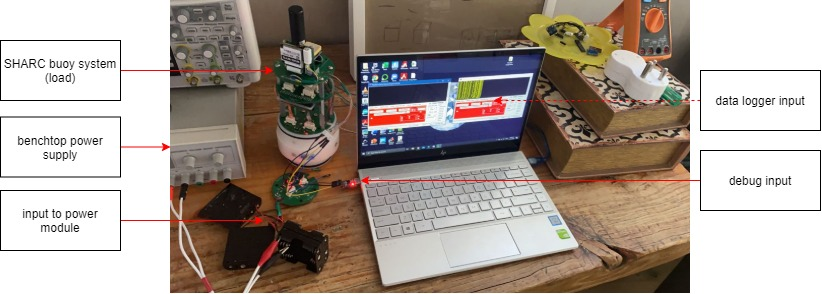
\includegraphics[width=\linewidth]{figs/pwrtest}
 	\caption{Diagram showing the configuration for the power test. All subsystems were connected and activated with version 2 sensors and firmware. Power was supplied by an Agilent xxxx bench top power supply set to a constant 7.2 V output. A data logger was connected to the INA219 sensor to sample the power information at a rate of 1 Hz}
 	\label{fig:pwrtest}
 \end{figure}
 

\subsubsection{Configurations}

The INA219 sensor sampled at 1 Hz while the drift measurements were sampled in intervals of 30 minutes, the IMU was set to a sample rate of 5Hz for 67.2 seconds. 
\subsubsection{Results}

Based on the test protocol outlined above, data was successfully collected over a complete buoy lifecycle. The current consumption characteristics for a constant load voltage are shown in Figure \ref{fig:test_pwr_cycle}. 

\begin{figure}[H]
	\centering
	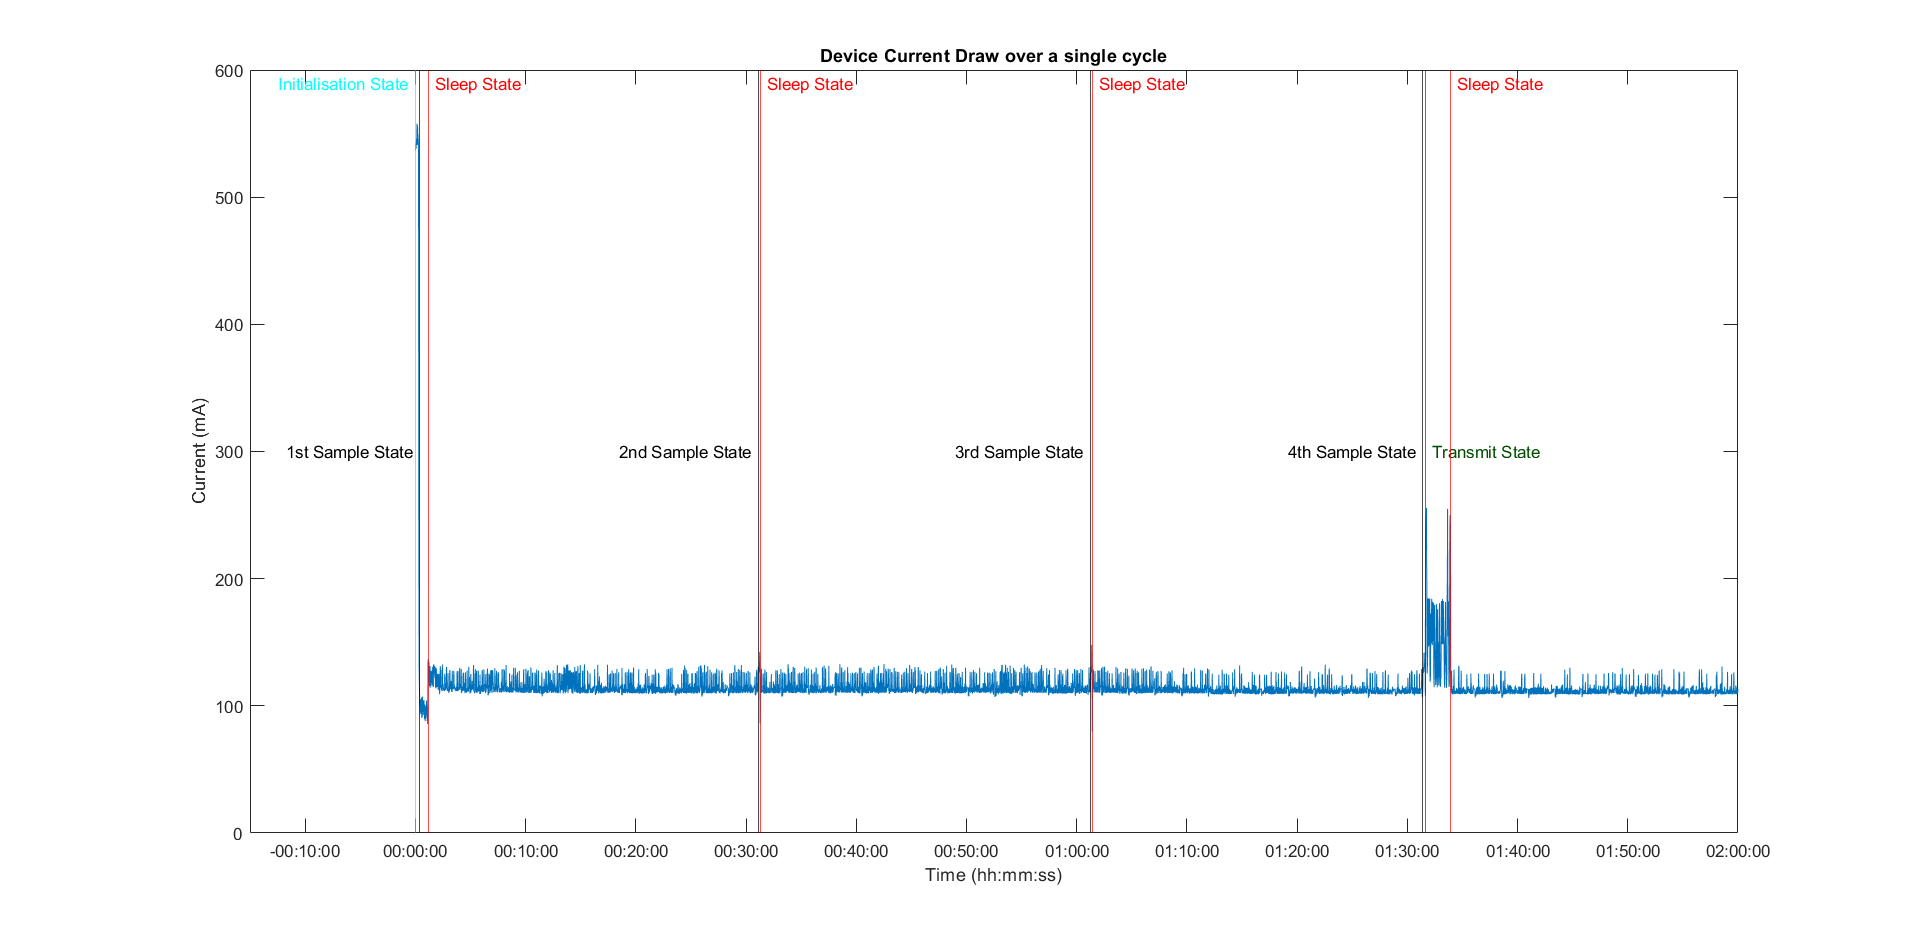
\includegraphics[width = \textwidth]{Power Cycle.png}
	\caption{Graph showing a typical current cycle of the buoy during the various phases. Data was sampled at 1Hz with all modules connected, sample intervals set to 30 mins the INA219 sensor connected to an external data logger and the device placed in a partially obstructed environment.}
	\label{fig:test_pwr_cycle}
\end{figure}


State transitions were captured through a debug serial monitor and timestamped to synchronise the state changes to the current draw as shown in Figure \ref{fig:test_pwr_cycle}. Then, the average current draw was calculated for each phase of the buoy with the period defined as the time between state transitions. The equation to calculate the average current is shown below.
\begin{equation}
	I_{avg} = \frac{1}{T}\int_{0}^{T}i(t)dt = \frac{1}{T}\sum_{k=0}^{N}i(k)\Delta t
\end{equation}

where the time step $\Delta t$ is 1Hz and $T $ is the total time taken for the buoy to complete 1 cycle. Then, The average current consumption and cycle duration was calculated for each phase in the buoy cycle. The results are shown in Table \ref{tab:test_powtest_data}.

\begin{table}[H]
	\centering
	\setlength{\extrarowheight}{5pt}
	\begin{tabular}{lcc}
		\hline
		\textbf{Cycle Phase: } & \textbf{Phase Duration (s):} & \textbf{Average current (mA):}\\
		\hline
		Initialization State & 20 & 494.37 \\
		\hline
		1st Sample State & 45 & 97.79 \\
		\hline 
		1st Sleep State & 1797 & 115.00 \\
		\hline
		2nd Sample State & 8 & 127.96\\
		\hline
		2nd Sleep State & 1797 & 114.41\\
		\hline
		3rd Sample Sate & 7 & 128.17\\
		\hline
		3rd Sleep State & 1797 & 112.87\\
		\hline
		4th Sample State (incl IMU) & 12  &129.71 \\
		\hline
		Transmit State & 135 & 157.01 \\
		\hline
		\hline
		Full Cycle:    & 10033 & 114.09 \\
		\hline
		\hline
	\end{tabular}
	\caption{Average current draw (mA) and cycle}
	\label{tab:test_powtest_data}
\end{table}
This shows that the buoy completes a cycle in 10033s (2 hours 47 minutes) which is 47 minutes longer than the predicted cycle. The average current conumption was 114.09 mA Finally, the average current consumption for each phase is displayed in Figure \ref{fig:test_powtest_avgcurr}.

\begin{figure}[H]
	\centering
	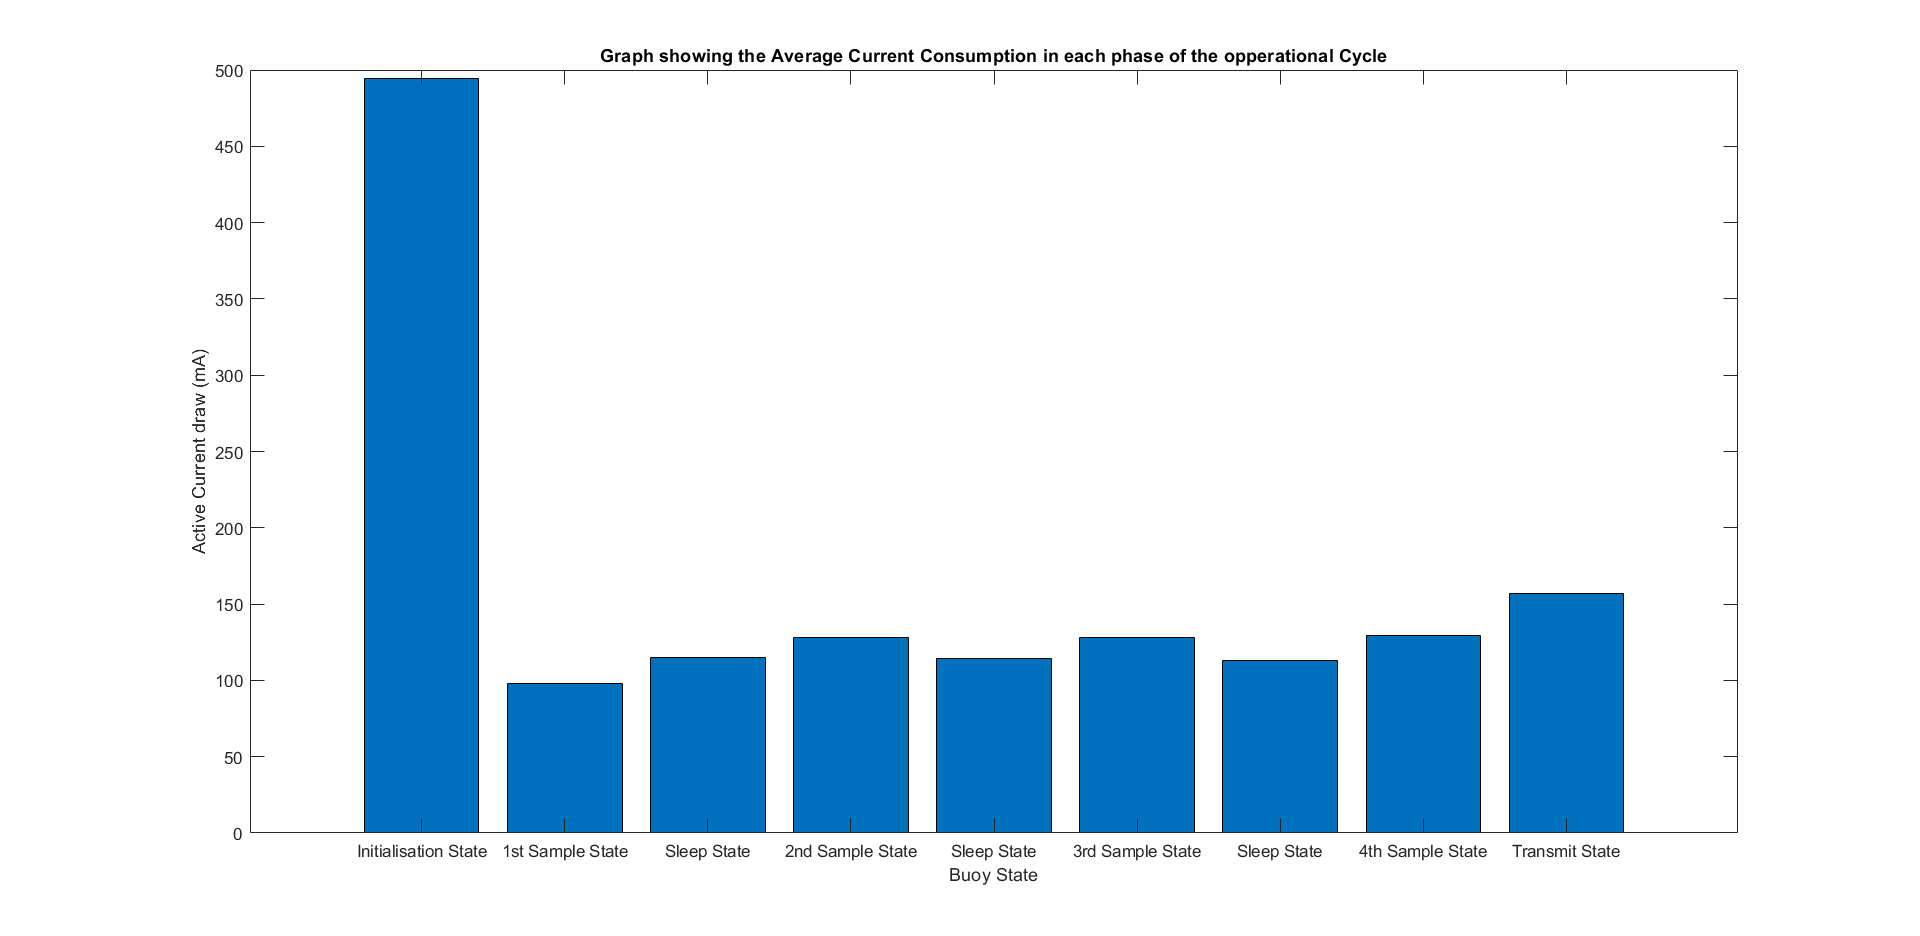
\includegraphics[width =\textwidth]{State Current Draw.png}
	\caption{Average Current consumption at each phase in the life-cycle of the buoy. Ordered chronologically}
	\label{fig:test_powtest_avgcurr}
\end{figure}

From Figure \ref{fig:test_powtest_avgcurr}, the longest current draw occurs at start up at 494.37 mA, the second largest current draw occurs during transmission (157.01 mA) while the lowest current consumption occurs during  the first sample state  (97.79 mA) with the sleep states drawing consistently the lowest current (112.87 mA to 115.00 mA).

\subsection{SYS003 low temperature test}

\subsubsection{Scope}

The low temperature test aimed to test the software performance in temperatures below 0$\degree$ C and verify this performance against AT007 (Table \ref{tab:AT007}). Successful completion of this test validates a critical user requirement of being able to withstand the climate of the Southern Ocean.
\subsubsection{Protocol}

All sensors were connected to the system and the Iridium modem was turned off. Sensors were set to the sampling intervals described at the begining of this section with the transmission routine removed from software. The device was powered with batteries and sealed with desiccant to prevent a build up of moisture. The device was placed in a commercial grade freezer to run for one hour saving data to the flash chips during its operation. The freezer was set to $-20\degree$ C and the buoy status was visually monitored. After the test, the buoy was placed in a room-temperature environment where another accelerated test SYS001 was performed.
\subsubsection{Configurations}

GPS set to timeout after 30 seconds, Sensors sampled in intervals of 30 minutes.
\subsection{Results}

During the test, the flash chip routine failed to save data resulting in all test data being lost.

\subsection{SYS004 field test}

\subsubsection{Scope}
goal is to deploy the system in a controlled environment to test that the system can complete a full cycle from start up to transmission. This test verifies the length of time the buoy can survive for as well as the transmission capabilities and measured data against AT009 (Table \ref{tab:AT009}).

\subsubsection{Protocol}
All subsystems were connected with GPS data,environmental data power consumption data and imu data enabled for transmission. Ice drift data was sampled in intervals of 30 minutes with IMU data sampled in intervals of two hours. Both IMU and ice drift data were transmitted after the fourth ice drift sample session in two seperate consecutive transmissions. The sensors were configured as shown in subsystem with version 2 of the SHARC buoy firmware and hardware. The device was connected to an array of batteries and placed in an environment with good line of sight of the sky. The device was left to run until no more transmissions were received. The device was then removed and the data was analysed.

\subsubsection{Configurations}
GPS messages sampled every 1Hz until a valid fix, timeout if no fix reached within 30 seconds. power sensor and BMP280 sensors sampled by triggering a measurement once during the interval. Flash chips set to circular buffer mode with the first available chip used to store data. 

\subsubsection{Results}

The data from the device was transmitted to the Rock Seven RockBLOCK data portal. Table \ref{tab:deployment_results} below shows the data logs downloaded from the data portal.

\begin{table}[H]
	\centering
	\caption{Data transmitted from the SHARC buoy as compressed binary messages in ASCII hexadecimal format. This table contains ice drift data shown in packets begining with 01 ("1") and IMU data in packets begining with 57 or "W". Also shown are diagnostic data including the transmitting device, payload size and number of credits used to transmit the message.}
	\label{tab:deployment_results}
	\setlength{\extrarowheight}{5pt}
	\resizebox{\textwidth}{!}{%
		\begin{tabular}{>{\raggedright\arraybackslash}m{2.5cm}>{\raggedright\arraybackslash}m{2.5cm}>{\raggedright\arraybackslash}m{2cm}>{\raggedright\arraybackslash}m{20cm}>{\raggedright\arraybackslash}m{2cm}>{\raggedright\arraybackslash}m{1cm}}
			\hline 
		\textbf{Date Time (UTC)} & \textbf{Device} & \textbf{Direction} & \textbf{Payload} & \textbf{Length (bytes)} & \textbf{Credits} \\ \hline\hline
		12/31/2020 7:51 & RockBLOCK 17285 & MO &\seqsplit{ 57022600e235f8d844ff84004602bc008e3642d2aeff70004c03c80162364cd2c1ff6b004d02ac01383690d2d3ff68004e0192010c3628d2e3ff68004e01f600023672d2f4ff60004f02f001583608d2fbff63004c0396004c37a2d30bff5e004c03dcfec036acd313ff5e004d039afeac3838d31dff58004a02aafef038a0d324ff5600480188fdf8393cd32fff5900430028fdf639a4d333ff5e004000eefd723a7cd33cff610039028afde23ab4d341ff670038034eff883ba4d347ff69003402e4ff383b36d344ff6e002f0142fcb43c2cd351ff78002c014efe723b3ad351ff7b002801c401e63c8ed357ff820024021402083bccd35cff82002101e000863bdcd35fff86002001eeffe43aead362ff89001b021001d23b5ed366ff87001e032c03de3ab8d367ff81001c0294043a3b2ed36cff81001b02ea01e639d6d36fff7b001c022c027a3a5ad372ff78001c0d} & 338 & 7 \\ \hline
		12/31/2020 7:51 & RockBLOCK 17285 & MO &\seqsplit{ 01008789ed5f51b2a2c524d1cb3c014f01a000622bb90000000d9a0100007c46bc158703eb010d019b90ed5f12e7a2c5eb909b3c012b01a0004f2fcc000000d5990100007c46b815ec0295010d02af97ed5fad1ca3c582a8db3e013a01a000532fdb000000ac990100007c46b8155303a3010d03c09eed5f2d52a3c5919b193f012301a0004c33e6000000a9990100007c46b41563030102} & 152 & 4 \\ \hline
		12/31/2020 5:50 & RockBLOCK 17285 & MO &\seqsplit{ 570526fd5c39dcd770ff49001203e6fd2437fed1b7ff3100130304fc2a3a56d1cdff3900190440fbd6384ed1e1ff40001b04b6fbf83932d1eaff44002403f0fce0396cd1f8ff4a002704defdbe3930d206ff52002c0404fc8839d0d213ff5a003203aafbd239f6d219ff620032043efc6439a0d223ff69003303fcfcb03b1ed22eff720036038efd4839aed235ff7a0038037cfb1e3b4ed23dff8300380232fa5438e4d246ff8800340186fb9a3a4ad247ff92003603ccfef039e6d24fff9800380320ff423a3ad24fff9d00370288fe6c39d2d256ffa6003602f0fe0438f2d25bffa9003403fafe943972d25effb200360382ff5239b8d261ffb30035033a010e38e0d265ffb70036039800c23a32d26fffb6003a026c01a838ead26effb4003c025602de39acd272ffb6003e03ca023c3956d275ffad0042038402123920d27bffac004200e6047e3992d27bffa600430d} & 338 & 7 \\ \hline
		12/31/2020 5:49 & RockBLOCK 17285 & MO &\seqsplit{ 0100e96ced5fb4a0a0c5022b073d015001a0005a2b740000002f9a0100007c46c815f60293010d010174ed5fcfd3a0c53aafb13d013e01a0005927710000004e9a0100007c46c4150f03c7010d02167bed5f2d07a1c5734babbc011900a000512b820000001d9a0100007c46bc15f302d7010d032b82ed5f8a3ba1c5d13f41bd012c01a00057279a0000002c9a0100007c46bc150703a301} & 152 & 4 \\ \hline
		12/31/2020 3:47 & RockBLOCK 17285 & MO &\seqsplit{ 57019c01423c82d6efff84001bff64fddc3cd4d127ff6a000ffcccfece3bd6d137ff6f0008ffac01a83b76d14cff6bfffe030404583cbad15bff69000303d402083b24d169ff6e000000d0fdee3a2ad179ff6dfffc0454023039fcd17fff680006057803c43a04d188ff63000905ba04303a16d194ff66001106f801303910d19aff650014045cffda37a2d1a1ff64001d0356ffd43736d1aaff5e0027056a00dc374ad1afff59002d05f00288382ad1b5ff57003904e8028e3734d1b9ff51003d023e02d43796d1c1ff4d003d02e6fff436a4d1c2ff4d003d02da02a037c6d1caff40004603ee01fc3714d1c9ff3d0043049e00043862d1cfff3400450236fdd036e2d1d4ff39004101a6fe3a3752d1d6ff340042016afc743832d1daff36004001a2fe7e38c0d1deff35003b01baff24385ad1dfff3d003700c6fe303910d1e0ff46003100c6fbf23820d1e4ff52002a0d} & 338 & 7 \\ \hline
		12/31/2020 3:47 & RockBLOCK 17285 & MO &\seqsplit{ 01006650ed5f4ae49fc5d2981641013301a0005d2768000000df990100007c46d4150103af010d017d57ed5f950da0c57b668140014401a0010b276a000000e8990100007c46d815ec02b7010d02945eed5f4d39a0c5ebe2363e020b01a001151f6d00000071990100007c46d015f702db010d03a865ed5f446ca0c5f41abb3b014d01a00060276e000000fd990100007c46d015f102af01} & 152 & 4 \\ \hline
		 \hline \hline
	\end{tabular}
	}
\end{table}

Table \ref{tab:deployment_results} shows a section of the data recieved during a deployment test. The data includes both IMU data (demarcated with a 0x57 or "W") and ice drift data (demarcated with a 0x01 or "1"). These payloads are compressed data packets as discussed in Chapter \ref{ch:ch5}

\section{Field testing}

This section describes the field testing performed during the 2019 SCALE winter cruise in July.This test occurred early in the development cycle and used version 1 of the software and the hardware for the SHARC buoy system. The cruise took place onboard the SA Aghulas II and followed a trajectory towards the Weddel sea shown in Figure \ref{fig:scalepath}. This system was deployed with sensors, processors and configurations shown in the table below.

\begin{figure}[H]
	\centering
	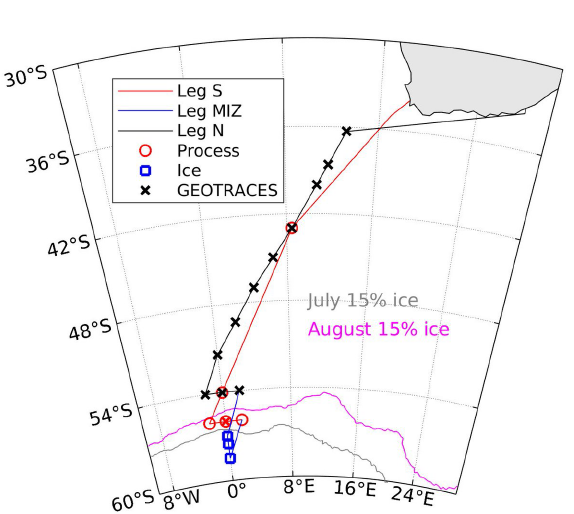
\includegraphics[width=0.7\linewidth]{figs/SCALEpath}
	\caption{Diagram showing the trajectory of the SA Aghulas II for the 2019 SCALE winter cruise from Cape Town to the Southern Ocean Marginal Ice Zone. Diagram created by E. Hepworth.}
	\label{fig:scalepath}
\end{figure}

\begin{table}[H]
	\centering
	\caption{Hardware components used  during field testing for version 1 of SHARC buoy deployed during the 2019 SCALE winter cruise to the Southern Ocean Marginal Ice Zone.}
	\setlength{\extrarowheight}{5pt}
	\begin{tabular}{ll}
		\hline
		\textbf{Subsystem} & \textbf{Component} \\
		\hline
	     GPS & u-blox NEO-7M \\
		\hline
	 Temperature sensor & DS18B20 \\
		\hline
		 Microcontroller & STM32F407VG \\
		\hline
		 Memory & Internal microcontroller flash memory \\
		\hline
	    Remote communication & RockBLOCK 9603  \\
		\hline
		\hline
	\end{tabular}
\end{table}

These components were connected to a double sided PCB and mounted vertically to the Base. The fully connected system can be seen in Figure \ref{fig:sharcv1}
\begin{figure}[H]
	\centering
	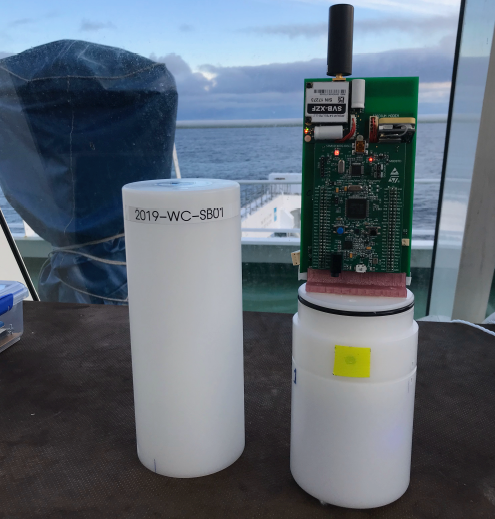
\includegraphics[width=0.7\linewidth]{figs/sharcv1}
	\caption{SHARC buoy version 1 used for deployment testing during the 2019 SCALE winter cruise in July. The device contains an Iridium modem, GPS and temperature sensor for sea ice drift and ambient temperature measurements. Photo by R. Verrinder.}
	\label{fig:sharcv1}
\end{figure}

Six prototype systems were brought onboard and carried to the Southern Ocean with the objective of testing the suitability, basic sensing capabilities, remote communication capability and GPS signal acquisition capabilities. During the expedition, the initial power system began to experience instabilities resulting in system failures. Due to time and resource constraints, alternative power supplies were made for three of the systems. Two systems were deployed in the first and second Marginal Ice Zone (MIZ1 and MIZ2) respectively, These locations can be seen in Figure \ref{label}. A final system was deployed on the helideck of the SA Aghulas II on the return journey to East London.

\begin{figure}[H]
	\centering
	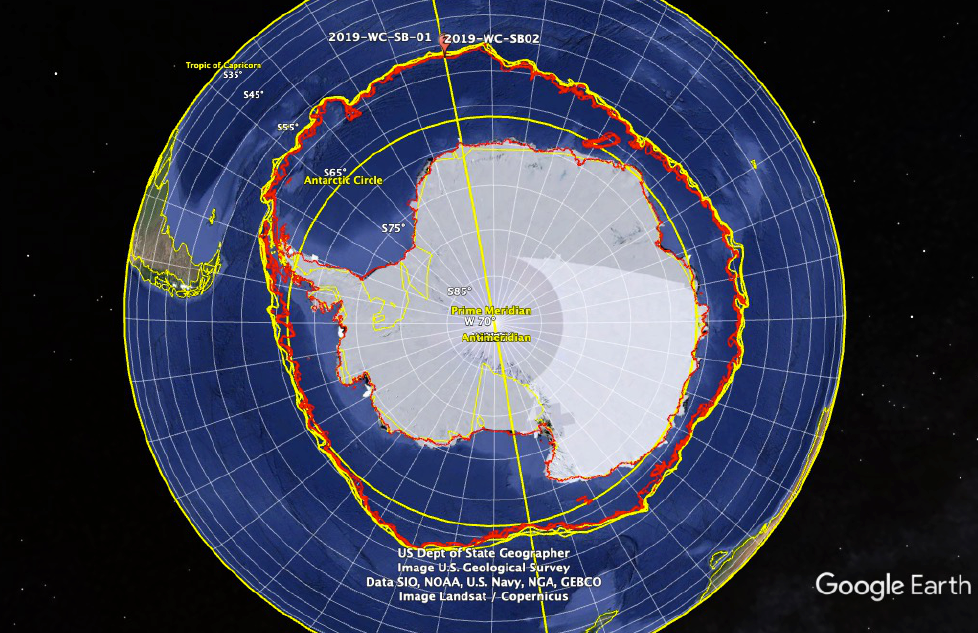
\includegraphics[width=\linewidth]{figs/deploc}
	\caption{SB01 and SB02 buoy deployment locations. Ice edge on 26 to 28 July 2019. Ice edge data provided by Ehlke from \url{https://www.natice.noaa.gov/products/ kml_daily.html}}
	\label{fig:deploc}
\end{figure}

\subsection{Configuration}
Before deplyoment, the system was testing using AT001 to AT004 for the subsystems and AT005 for the full system. Low temperature validation was performed on the deck of the ship while near the Southern Ocean. The device was configured to sample GPS and temperature data in intervals of 30 minutes with a single triggered temperature measurement and A GPS reading every 1 Hz until a signal was acquired. The configuration parameters are shown below.

\begin{table}[H]
    \centering
    \caption{Table showing the parameters the GPS was configured with before deployment. }
    \begin{tabular}{lc}
    \hline
    \textbf{Model:} & Ublox Neo-7M \\
    \hline
       \textbf{Baud Rate:}  & 115200 bit/s \\
       \hline
       \textbf{Data bits:} & 8 \\
       \hline
       \textbf{stop bits:} & 1 \\
       \hline
       \textbf{parity:} & None \\
       \hline
       \textbf{Active Networks:} & GPS, GLONASS \\
       \hline
       \textbf{Satelites:} & 3 to 6 \\
       \hline
       \textbf{NMEA Messages:} & GLL, GSA, ZDA \\
       \hline
    \end{tabular}

    \label{tab:test_remotetest_gpsconfig}
\end{table}

\subsubsection{Deployment protocol}

The buoy was switched on and sealed in the enclosure which was fastened to the buoy stand and placed on the deck of the ship. The buoy was placed in a personnel basket along with three crew members who were fastened to the basket with personal harnesses. The basket was attached to a crane, hoisted over the side of the ship and lowered towards the surface of the ocean. The crew members then identified a suitable ice floe to place the buoy on. The floe had to have a diameter greater than 2 m and visually capable of supporting the weight of the buoy (i.e. no visible rafting or flooding). Once an ice floe was selected, the basked was maneuvered to hover 1 m above the desired location. Figure \ref{fig:deployment} shows the deployment of the buoys in the Marginal Ice Zone using this procedure. 

\begin{figure}[H]
	\centering
	\begin{subfigure}[t]{0.3\textwidth}
		
		\begin{tikzpicture}
			\node[anchor=south west,inner sep=0] (image) at (0,0) { 		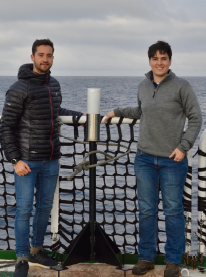
\includegraphics[width = 0.95\linewidth,height=6cm]{SHARCv1full.PNG}};
			\begin{scope}[x={(image.south east)},y={(image.north west)}]
				\draw[color=black, ultra thin,fill=white] (0.0,0.0) rectangle (0.16,0.16) node[pos=.5] {A};
			\end{scope}
		\end{tikzpicture}

	\end{subfigure}%
	\begin{subfigure}[t]{0.3\textwidth}
		\begin{tikzpicture}
			\node[anchor=south west,inner sep=0] (image) at (0,0) { 		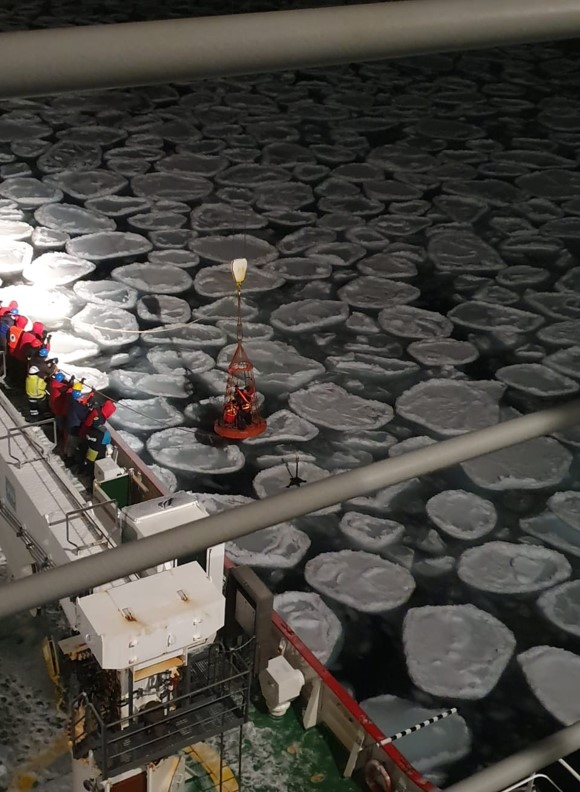
\includegraphics[width = 0.95\linewidth, height = 6cm]{basket.jpg}};
			\begin{scope}[x={(image.south east)},y={(image.north west)}]
				\draw[color=black, ultra thin,fill=white] (-0.01,0.0) rectangle (0.13,0.13) node[pos=.5] {B};
			\end{scope}
		\end{tikzpicture}

	\end{subfigure}%
	\begin{subfigure}[t]{0.3\textwidth}
	\begin{tikzpicture}
		\node[anchor=south west,inner sep=0] (image) at (0,0) { 		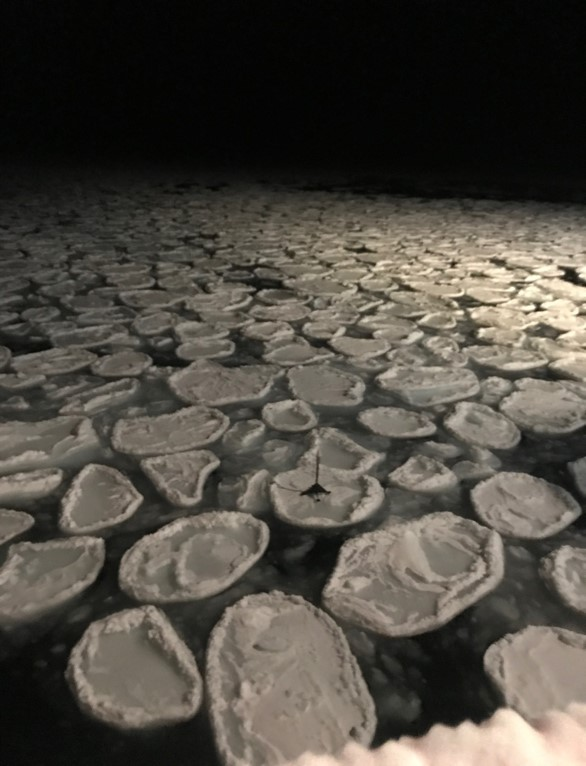
\includegraphics[width = 0.95\linewidth, height = 6cm]{deployment.jpg}};
		\begin{scope}[x={(image.south east)},y={(image.north west)}]
			\draw[color=black, ultra thin,fill=white] (-0.01,0.0) rectangle (0.13,0.13) node[pos=.5] {B};
		\end{scope}
	\end{tikzpicture}
	
\end{subfigure}%
	\caption{Photos taken during field testing of the SHARC buoy system showing (A) the device fully assembled and secured to the stand (photo: R. Verrinder), (B) the device deployed onto an ice floe via a basket and crane deployment procedure, (C) SHARC buoy on an ice floe following a successful deployment. }
	\label{fig:deployment}
\end{figure}

The buoy was then deployed from the basket with enough force for the spikes to penetrate into the sea ice thereby tethering the stand to the ice floe. Once complete, the buoy tracked GPS coordinates, signal diagnostics, datum information and ambient temperature. The conditions of the deployment are shown in the table below.
\begin{table}[H]
    \centering
    \caption{Deployment conditions for buoy 1 (2019-WC-SB01) and buoy 2 (2019-WC-SB02) including deployment coordinates, time and environmental conditions}
    \setlength{\extrarowheight}{5pt}
    \begin{tabular}{lll}
    \hline
    \textbf{Buoy serial number} &\textbf{ 2019-WC-SB01} & \textbf{2019-WC-SB02}\\
    \hline
    \hline
    Latitude & $56\degree 59'59.70"$ S& $57\degree 17'11.28"$ S\\
    \hline
    Longitude & $0\degree 0'36.96"$ E& $0\degree 1'18.30"$ E\\
    \hline
    Date & 26th July 2019 & 28th July 2019\\
    \hline
    Time [UTC] & 22h15 & 03h15\\
    \hline
    Air temperature [$\degree$ C]& -10.7  & -17.5\\
    \hline
    \hline
    \end{tabular}

    \label{tab:test_remotetest_Deployemt }
\end{table}

\subsubsection{Results}
\label{sec:ch4_results}

SB-WC-01 transmitted one message after deployment before losing contact possibly due to a power system failure. SB-WC-02 failed to transmit any messages which may have been due to mechanical failure as a result of deployment. SB-WC-3 survived on the helideck for one week until the batteries were changed. The buoy continued to transmit data continuously. GPS data collected from the transmission packets was compared to the GPS data recorded from the ship and the results are shown in Figure \ref{fig:test_deploymenttest_GPS}.

\begin{figure}[H]
	\centering
	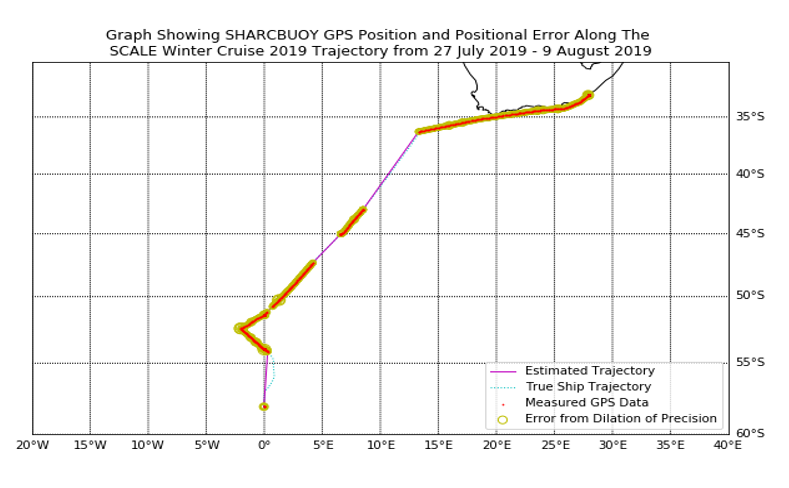
\includegraphics[width= \textwidth]{gps_trajectory_scale2019.png}
	\caption{The GPS trajectory of the SA Aghulas II ship from the Marginal Ice Zone to East London. The plot shows the estimated position (magenta) taken from the buoy samples (red) compared to the actual trajectory (cyan). The positional error (PDOP) of each measurement is shown as an exaggerated area around the measured position.}
	\label{fig:test_deploymenttest_GPS}
\end{figure}

Figure \ref{fig:test_deploymenttest_GPS} shows the measured GPS trajectory closely matched that of the ship however, there were significant gaps in the data set which was attributed to loss of GPS signal or failed Iridium transmissions. The dilation of precision appears the highest between 50 $\degree $ S and 55 $\degree $ S. As discussed in Section \ref{sec:ch2_drift}, this source of error may be attributed to strong ionospheric interference and poor satellite spread.

Finally, Figure \ref{fig:test_deploymenttest_temp}  shows the ambient temperature sampled by the buoy during its journey from Antarctica to East London. The data collected was compared to the data from the ship's on-board weather station.

\begin{figure}[H]
	\centering
	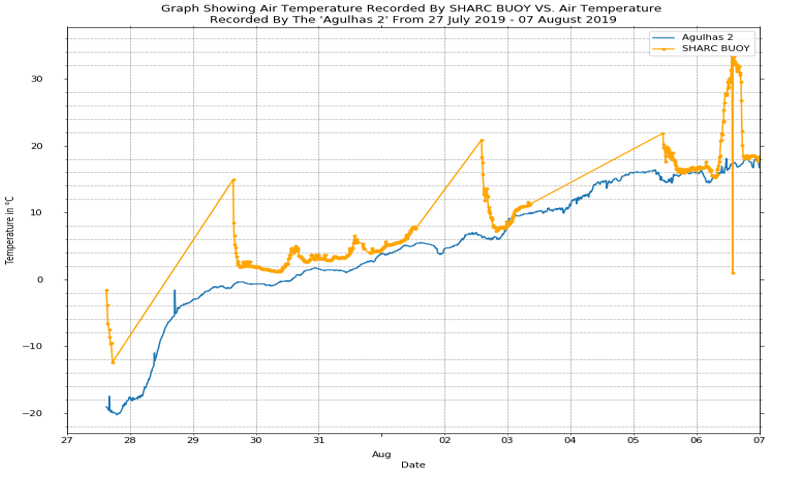
\includegraphics[width= \textwidth]{temp_test_scale2019.png}
	\caption{Air Temperature recorded by the buoy (yellow) over 11 days compared to the air temperature recorded by the ship (blue) }
	\label{fig:test_deploymenttest_temp}
\end{figure}

Figure \ref{fig:test_deploymenttest_temp} shows that the temperature sensor readings do not correlate at all with the reading from the ship. Furthermore, the gaps in the data sets lead to "spikes" appearing. The DS18B20 was not calibrated before deployment which may have caused these readings. Furthermore, the DS18B20 may have been unresponsive when the GPS signal was active resulting in missing data points. Finally, while the data points are inaccurate at low temperatures, the data trends towards higher temperatures as the ship reached higher latitudes. This trend was confirmed in the temperature measurements of the SA Aghulas II showing that the device was functional but very inaccurate.

\section{Final evaluation}
\label{sec:ch4_final_eval}

In this section, the results of the platform system and subsystem tests are discussed. Due to timeline constraints, no calibration testing was carried out other than for the INA219 current sensor where this was necessary for the device to function. On a full system level, the results of the acceptance tests are shown in Table \ref{tab:AT_SYS_EV}
\begin{table}[H]
    \centering
    \caption{Results of the full system acceptance tests indicated by a tick in the appropriate column.}
    \setlength{\extrarowheight}{5pt}
    \begin{tabular}{cccc}
    \hline
    
    \multicolumn{1}{c}{}&  \multicolumn{3}{c}{\textbf{Full system acceptance}} \\
    \hline
    \hline
    \textbf{Test ID} & \textbf{Fully satisfied} & \textbf{Partially Satisfied} & \textbf{Not satisfied} \\
    \hline
   \hline
    AT006 & & \checkmark & \\
    \hline
    AT007 & \checkmark & & \\
    \hline
    AT008 & &  \checkmark& \\
    \hline
    AT009 & & & \checkmark \\
    \hline
    \hline
    \end{tabular}

    \label{tab:AT_SYS_EV}
\end{table}

Full system calibration was partially satisfied. The power monitor circuit was calibrated successfully for the power supply and the IMU successfully passed the self-test. However, extensive IMU calibrations could not be performed. The extent of IMU functionality demonstrated by this platform is to prove functionality by initialising and sampling at a fixed known rate. Furthermore, long-term data logging and wave measurements fall outside the scope of this project. It is recommended for future research to create an acceptance test for extensive IMU calibrations. Finally pressure measurements are difficult to verify without a calibrated barometer. In future work, verification of the environmental sensor should be conducted at a location with a calibrated weather station.

The system  completed low temperature tests in a -20 $\degree$ C freezer and could function normally afterwards. However, due to an issue with the flash chips, all data from the test was lost. The only indication the buoy was operational was through a debugging LED.In the future, more extensive low temperature tests should be conducted. An additional improvement is to link the device to a data-logger and conducted low-temperature data validation tests to ensure proper operation of the buoy in low temperatures.

\subsection{Functional requirement validation}
Once the testing was completed, the system was evaluated against the system requirements. This section shows how the functional requirements were satisfied in the context of the overall project to increase remote sensing in the Southern Ocean. This ultimately proves if the steps undertaken in Chapter \ref{ch:ch3} had successfully fulfilled the requirements outlined by the stakeholders and evaluate the achievements of the device. These results are shown in Table \ref{tab:final_eval_funcreq}.

\begin{table}[H]
    \centering
    \caption{Results of the platform evaluation and how each functional requirement was addressed.}
    \setlength{\extrarowheight}{5pt}
    \begin{tabular}{m{0.15\textwidth}l m{0.7\textwidth}|}
    \hline
     \textbf{Functional requirement}   &  \textbf{Validation} & \textbf{Discussion}\\
     \hline
     \hline
     FR001 & Fully met & \textit{The system shall have a protective enclosure against precipitation and frost.}\\
          \hline
     FR002 & Fully met &\textit{Enclosure shall be from strong, corrosion resistant materials with strong thermal characteristics}. This requirement was validated from the deployment tests during the 2019 SCALE Winter cruise. The buoy continued to transmit during rain, ocean spray and low temperatures thereby providing sufficient protection to the electronics.\\
          \hline
     FR003 & Partially met& \textit{The device will protect electronics from internal humidity} - This requirement was partially met. When the device transitioned from sub zero temperatures to room temperature, condensation formed both inside and outside the device. While the electronics continued to work, this could result in unexpected failures and needs to be addressed in the next iteration.\\
          \hline
     FR004 & Fully met. & \textit{The electronics will be elevated above the ground by 1 m.} The buoy stand reaches 1.2 m to satisfy thsi requirement. \\
          \hline
     FR005 &Fully met & textit{All subsystems shall be rated for extreme temperatures}. This was an inherrent requirement for component selection which was validated with acceptance test AT005 (Table \ref{tab:AT005}). The devices would not have been included if this requirement was not met.\\
          \hline
     FR006 &  Fully met &\textit{System will transmit data via Iridium satellite network.} Data was received through the Rock Seven RockBLOCK data portal thereby validating remote communication capabilities.\\
          \hline
     FR007 & Fully met &\textit{Device shall be battery powered.} The device successfully survived for days on a single battery charge in low temperatures. \\
          \hline
     FR008 & Fully met &\textit{Device shall measure ice drift using a global positioning system (GPS). The GPS module successfully acquired satilite signal and produced time stamped coordinates. The average DOP was measured to be 5 below latitudes of $50 \degree$ S which, according to Table \ref{tab:gps_DOP} is a good measurement accuracy.}\\
          \hline
     FR009 & Partially met& \textit{Device shall measure ambient temperature}. The BMP280 could not be verified in low temperatures. The DS18B20 produced wildly inaccurate values as it was not calibrated properly.  \\
          \hline
     FR010 & Partially met & \textit{Device shall measure atmospheric pressure}. The BMP280 produced a pressure reading however the device could not be verified in low temperatures.\\
          \hline
     FR011 & Partially met. &\textit{Device shall contain an inertial measurement unit (IMU) to record acceleration (3-axes) and rotation (3-axes) of an ice floe.} - A proof of concept was implemented with the IMU capable of sampling all 6 axes for a total of 336 bytes of data. This is an insufficient to calculate significant wave height.\\
          \hline
     FR012 & Fully met & \textit{Device to contain sufficient memory for data storage}. The four flash chips have a total storage space of 8 MB. As shown in Section  \ref{sec:dm}, the chips have sufficient storage space to store 152.19 years worth of drift data which is enough to cover a seasonal cycle \cite{barber2005microwave}. Th chips can store37 days worth of raw IMU data sampled at 5 Hz for 20 minutes. Which allows for similar data collection periods experienced by \textcite{kohout2015device} who additionally implemented processing. \\
          \hline
     FR013 & Fully met &\textit{ Device to contain a processing unit to control sensors and process data.}\\     
     \hline
     FR014 & Fully met & \textit{ Device to be optimised for low-power consumption and power event handling}. The buoy successfully entered low power mode during periods of inactivity which resulted in a lower current draw than the other phases.\\
          \hline
     FR015 & Unsatisfied & \textit{Device shall be factory calibrated prior to shipping and delivered in a state where it can be deployed at a moment's notice.} The device entered the main loop and started running as soon as the power was on. However, the sensors were insufficiently calibrated to fully meet this requirement.\\
          \hline
    FR016 & Fully met & \textit{Device will cost less than currently available systems.} - The overall cost for a single system is R8,421. From the review of remote sensing devices, a comparison of device cost is shown in Table \ref{tab:device_price}. From this comparison, the SHARC Buoy is much cheaper than  WIIB \cite{rabault2019open} which costed R30,200 and had similar features. However, this device used more reliable components and implemented more complex data processing strategies resulting in better wave estimation calculations than the SHARC buoy. \\
    \hline
    \hline
    \end{tabular}

    \label{tab:final_eval_funcreq}
\end{table}

\section{Discussion}
\label{sec:ch4_disc}

\subsection{Power requirements}
\label{subsection:PWR}
The Initialization state was the most power intensive state drawing 494.37 mA. This was attributed to the Rock Seven Rockblock 9603 modem which has a reported startup current of  450 mA to charge the on-board super capacitors. The effects of placing the modem to sleep can be seen throughout the data in Figure \ref{fig:test_pwr_cycle} and Table \ref{tab:test_powtest_data} where the average current barely increases above 130 mA. The effects of putting the buoy to sleep mode when the device is inactive results in a significant drop in current consumption as the average current consumption during sample mode was roughly 10-15mA larger than the current consumption during sleep mode. However, this is not true for the first sample state which results in the lowest current consumption at any point in the operational cycle of the buoy. However, since this phase occured so close to the power up of the buoy, it may have been a result of the GPS searching for satelite signal which consumes less current than when in acquisition state \cite{UBLOX_M7N_DATA}.\par 

The fourth sample state had the largest average current draw and the longest phase duration of all the sample states. This was to be expected as the inclusion of IMU sampling results in a longer data acquisition time as well as a higher current consumption. Finally, The transmission phase was expected to have the second highest current consumption since the Iridium modem was turned back on. At this point, the current draw increased to 250 mA as shown in figure \ref{fig:test_pwr_cycle}and occurred twice during the transmission phase. Despite this spike in consumption, the average current over the transmission phase was 157.01 mA despite multiple transmission attempts.\par 

The duration of each state has a significant impact on the average current consumption of the buoy. While the initialization state current and the Transmission state had significantly higher current consumption, the phase duration of these states were significantly smaller than the sleep states. The long periods of inactivity dominated the power cycle resulting in an average current of 114.09 mA. The duration of the sample states were small as a result of fast data acquisition and sampling speeds. However, the first sample state had the longest duration. This was due to a failure to acquire a GPS signal within 30 seconds which resulted in a timeout. The fourth Sample state also had a relatively long phase duration due to the inclusion of the IMU in the sample routine. Finally, the longest, active state was the Transmit State. During this state, multiple attempts were made to successfully transmit a packet of data and failed resulting in the relatively long phase duration. Overall, it took 10033 seconds or (2 hrs 47.217 min) whereas each sleep state was found to be extremely consistent. This shows that the sample and transmit states have a non-negligible duration which can affect the accuracy of the sampling resulting in time delays and desynchronisations. These can be attributed to sensor measurement time, GPS signal acquisition time, and the Iridium transmission time which runs for 10 minutes. Furthermore, the sleep periods were set using fixed, full time periods counting from when the sample phase is concluded. Therefore, to account for this, the system must measure the time taken between wake up and the end of the sample phase and remove this from the inactive period counter to synchronise the sample state to the required sampling interval.

\subsection{System performance}

To verify the sensor accuracy during the deployment test. Time, data, temperature and positional data sampled at 1 minute intervals was acquired from the SA Aghulas II. Figure \ref{fig:test_deploymenttest_GPS} shows that data collected from the buoy's GPS correlated well with the data from the ship. However, large gaps appear in the buoy's data-set. This can be attributed to signal loss or failure to acquire GPS position. In addition. the positional error appears larger for coordinates greater than $50\degree S$ and smaller as the trajectory approaches East London. This could suggest that the GPS satellite signal is much weaker closer to the Antarctic continent and may be attributed to either the strength of the antenna or the spread of GNSS satellites in the region.

Figure \ref{fig:test_deploymenttest_temp} shows that the temperature measured by the sensor was wildly inaccurate. However, the sensor was not calibrated before deployment which resulted in the inaccurate measurements. Additionally, Missing packets resulted in large "spikes" in the data. The data, however does show a trend towards warmer temperatures which is also reflected by the ship data. Therefore, the sensor was able to characterise the change to warmer temperatures however, the data is too inaccurate to be valid. This data from version 1 of the buoy was captured with the DS18B20 thereby showing it was not practical for this application. The new sensor (BMP280) could not be verified by remote testing due to cancellations of the 2020 Antarctic expedition.

\subsection{Mechanical features}

The mechanical features of the system successfully met the functional requirements FR001, FR002, FR004. FR003 was partially met as preliminary freezer tests resulted in condensation both inside and outside the system. In spite of this, the electronics continued to work. However, a revision of the design should be made to reduce the internal humidity of the system when it transitions from a sub-zero environment to room temperature. \par 

The mechanical features of the system, while robust, were quite bulky and heavy. The stacked PCB design allowed for robust, modular development of the system and resulted in increased mechanical strength. However, the result was increased physical size of the device and increased cost. For future iterations, a single PCB with all the components should be created. By reducing reliance on off-the-shelf development boards, the performance, size and power consumption of the system can be more carefully controlled. More over, a single PCB design requires less physical hardware to secure the system to the enclosure such as hex spacers, screws and washers. This can significantly reduce the price of fabrication. This design was also found to create points of failures within the device. By having separate PCBs, additional wires were required to connect the boards. If a wire loses contact or breaks, the device stops working. Finally, by reducing the electronics size, more batteries could be included which can provide more power for the system.

\subsection{Power system}

The power system was the largest constraint to the device. The physical size of the enclosure limited the number of batteries included in the system and therefore lifespan of the buoy. The initial decision was to use LiSoCl$_2$ D cell batteries. These were chosen for their high specific energy and low temperature resistance. Two 3.6 V batteries were connected 2 in series and 2 in parallel resulting in 7.2 V into the LDO. However, in low temperature environments, the internal resistance of the batteries dropped significantly resulting in system brownouts and unexpected resets. These were exchanged for AA LiFeS$_2$. These batteries had higher stability at lower temperatures at a cost of significantly reduced specific energy. In addition, four cells were required in parallel to produce the required voltage thereby increasing the battery requirement.\par 

The result was a maximum survivable period of 8 days in low temperatures $< 0 \degree $ C and 10 days in standard temperature. The seasonal requirement for operation is at least a month. To meet this requirement, the power system requires significant revision. The average load current was estimated to be 114.09 mA over a two hour cycle.  The total energy requrement $114.09 \times (30 days) \times (24 hours)$ or $82,114.8$ mAh for a period of thirty days. Future improvements to meet this requirement would be to use batteries with higher specific energy, couple the power system with an energy harvester or use a rechargeable power source. Additionally, the load current can be reduced significantly by implementing more power saving features such as MOSFET switches to turn off unneeded sensors or configuring devices such as the GPS for power saving mode.

\subsection{Future work on wave measurements}

Section \ref{sec:ch1.section1} shows that waves in ice  strongly affect the  formation and dynamics of sea ice in the Southern Ocean. \Textcite{vichi2019effects,albarello2020drift,kohout2015device,rabault2019open} also show the importance of increasing remote sensing of waves in the Marginal Ice Zone. Therefore, for this project, IMU integration was a fundamental step. The IMU was successfully integrated into the project. However, the sampling requirements resulted in extremely large data sets requiring complex data management algorithms. Morever, the constraints of the Iridium data buffer significantly impacted the type of data that could be transmitted. The recorded time series requires compression algorithms/software processing algorithms which fall outside the scope of this thesis. Therefore, in terms of the project goals, the IMU only partially satisfies the requirements and more firmware development is required for wave data measurements to become fully realisable.

The MPU6050 is a low cost, 6 axis inertial measurement. This more than satisfies the requirements for analysing waves in terms of spectra, co-spectra and significant wave height as shown by \textcite{kuik1988method} and \textcite{earle1996nondirectional}. The majority of devices in the field use high precision, expensive IMUs with low cost devices similar to the MPU6050 to verify the measurements. This shows that there is still room for investigation into the accuracy and performance of low cost IMUs for complex functions. 

\subsection{Short-burst data modems vs Telephone modems}

The current version of the SHARC buoy uses a short-burst data modem with a maximum transmission buffer size of 340 bytes. This resulted in extreme data constraints which reduced the functionality of the system. Despite this complexity, the device was well integrated into the system and was able to reliably transmit data even through the enclosure. Short Burst Data is a very data limiting protocol and is not a feasible solution for real-time, raw IMU data transfer. In future version, the Iridium 9522A would be a more feasible solution as the data buffer is much larger (1960 bytes). Alternatively, an Iridium device with a SIM card or continuous real time data transmission protocol.\par

The modem required the most design consideration. The device dominated the current sample and had the highest current consumption of all components. Hence, the majority of software optimisation was focused on optimising the power cycle of the device. Despite having an extremely large current cycle, the average current consumption over a two hour cycle was reduced significantly therefore successfully meeting the functional requirements.

\subsection{Evaluation against the State of the Art}

The final evaluation for the system was against other devices in the field. Most of these devices have been field tested to a larger extent than this device and have a higher technological readiness level. Significantly more testing is required to verify the field performance against the operation of the system.\par

However, SHARC buoy consumes significantly less power than the majority of devices in the field. The mode supply voltage is 12 V with some devices drawing up to 18 V compared to the buoy's 7.2 V operating voltage.\par 

Finally, while the SHARC buoy has more primitive modules on board, the device can, more evenly, measure a wider range of variables. Most devices generate complex measurements from single modules such as a high-powered IMU or AHRS measurement system. Devices such as WIIOS and WII buoy only contain low powered modules to compliment the measurements of the higher-powered components. This provides a unique opportunity for SHARC buoy to provide a deeper insight into performance optimisation in this region.\par 

Overall, the system shows that it is unique and fits a niche as a low powered, modular sensing device however, more rigorous tests and calibrations are required to bring the device to an overall state of technological readiness.

\section{Conclusion}

In conclusion, the device was evaluated on a unit level, a subsystem level and a full system level to verify the functionality against the user requirements. Field testing was conducted during the SCALE winter cruise where the device performance was tested in unknown conditions to determine the viability of the device in the Southern Ocean climate.